\chapter{CCD and Detector Parameters}
In this chapter, I will deal with some miscellaneous but important topics about CCD or other types of detectors (e.g., there is no available CCD in infrared wavelength, so technically they're not CCD). 

\section{Calibration Frames}
There are mostly three types of calibration frames in observational astronomy: bias, dark, and flat. Others inlcude comparison arc lamp images, various types of flat (dome, sky, etc). In this section, I referred HowellSB (2006) ``Handbook of CCD Astronomy'' 2e, chapter 4. 

\subsection{Detector Readout}
To understand why we need the bias, which is a technical than scientific reason, we need to know how the detector is being read out, so I separated this part from the \cref{ss: calib-bias}. When a CCD is being read out\footnote{It is assumed you know how the CCD or photodetectors transfer electrons; if not, search for, e.g., CCD clock pattern.}, the electronics need to convert the number of (photo-)electrons into a digital unit (so-called ADU or DN), where the number of ADU is, by the definition, number of electrons divided by the electron gain. 

But how can it count the number of electrons? Consider we have a voltmeter, attached to the `measuring position' (the output gate). By the clock pattern of CCD, the \textbf{correlated double sampling} (CDS) process is done as follows:
\begin{enumerate}
  \item Reset the output gate's voltage: $ V_\mathrm{out, 1} = V_\mathrm{reset} $.
  \item Measure $ V_\mathrm{out} $.
  \item Dump the electrons to the output gate, so the voltage will change by $ V_\mathrm{e} $.
  \item Measure the output gate's voltage again $ V_\mathrm{out, 2} $ (which is now $ V_\mathrm{reset} + V_\mathrm{e} $)
  \item Get $ \Delta V = V_\mathrm{out, 2} - V_\mathrm{out, 1} = V_\mathrm{e}$ (trivially the number of electrons is linearly related with this)
  \item Iterate this again and again until all the pixels are read out.
\end{enumerate}
The $ V_\mathrm{e} $ is then converted to ADU or DN by the Analog-to-Digital Converter (ADC). 

What I want to emphasize here is that the processes number 1 (resetting) and 4 (dumping) are not perfect, so the voltage over time ($ V(t) $) graph is never a combination of linear lines as in \cref{fig:cds}. The resetting and dumping involves movement of electrons, which results in a damped oscillation in the $ V(t) $ graph. If we had plenty of time, we can just wait until it stablized; however, we need to read out pixels as soon as possible (consider reading out 1000 by 1000 pixel CCD: to read out it in 1 sec, we need to read each pixel in $ \SI{1}{\mu s} $!). If it takes long time, you may lose observation time, and the dark current at the first-read pixel and the last-read pixel may differ, etc. Therefore, it is impossible to avoid the \emph{readout noise}. For some CCDs, there are options you can choose to compromise these readout time and readout noise. 

\begin{figure}
\centering
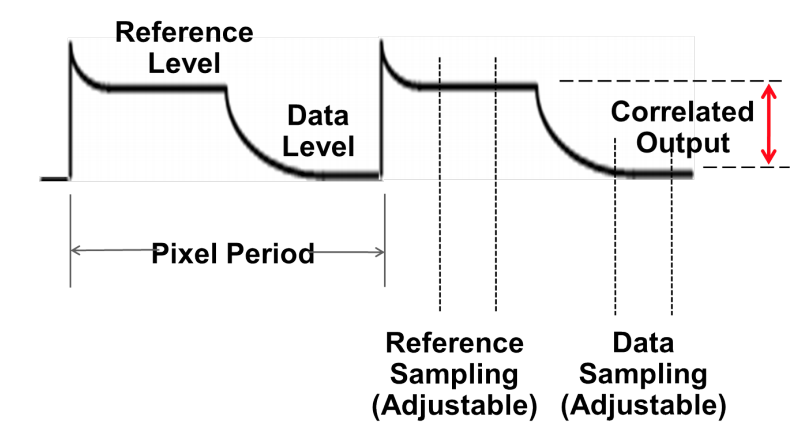
\includegraphics[width=0.5\linewidth]{figs/CDS}
\caption{CCD output and correlated doubling sampling. The vertical axis is the voltage and horizontal axis is time. You can see the voltage is not a combination of linear line segments, but noisy curves. (Image from Texas Instruments, 2018: \href{ti.com/lit/an/snaa322/snaa322.pdf}{ti.com/lit/an/snaa322/snaa322.pdf})}
\label{fig:cds}
\end{figure}


\subsection{Signed and Unsigned \texttt{int}}
In computer science, there are two ways to express integers: signed and unsigned. For instance, an 8-bit integer of number 3 can be expressed as \texttt{0000 0011}. How about negative 3? \texttt{1000 0011}. That means, the first part of the 8-bit is used as \emph{sign}. From this sense, an 8-bit integer can express from $ (-2^7) = -128 $ to $ (+2^7-1) = +127 $. But in astronomical science, we know there should be no negative pixel value, and therefore there is absolutely no need to use the first bit as sign bit. Then we can store the numbers from $ 0 $ to $2^8 - 1 = 255 $, called the \emph{unsigned} integer format. Thus we could express almost double amount of data (twice the resolution) without losing any storage.

Although astronomers use \texttt{BZERO} and \texttt{BSCALE} technique in the FITS file format in reality, the idea is similar to unsigned integer. The output images are frequently \textbf{assumed to have no negative pixel values}. This is one of the reasons why we need the bias frame, explained a bit more in \cref{ss: calib-bias}.



\subsection{Bias} \label{ss: calib-bias} 
\begin{defn}[Bias]
A \textbf{bias frame} is ideally a frame with neither source signal nor thermal electrons. In practice, it is obtained with 0-sec (or the shortest possible) exposure time with shutter closed.
\end{defn}

Now you know we have to go with readout noise; we cannot remove it. As technology improves, the readout noise $ R $ decreased down to only few electrons per readout. Early days when CCD was first used in astronomy, it was at least tens of electrons (e.g., $ R \sim \SI{50}{e} $, and it's still true in infra-red detectors), or up to hundreds of electrons. Since gain is $ \sim 1\mathrm{-}10 \,\mathrm{e/ADU} $, that means each pixel might have at least $ \pm $ tens of ADU uncertainty. Thus, even if you take a bias frame, which must have nearly a constant value $ b $, you may have a Gaussian distribution of, e.g., $ \mathcal{N}(b, 10^2) $. 

Consider a 1K by 1K CCD with bias follows Gaussian of $ \mathcal{N}(b, 10^2) $. You have $ 10^6 $ pixels, and if you observe for 1 year, you may have taken $ 10^5 $ to $ 10^6 $ frames, which translates into the number of pixels read out per year of $ 10^{10} $ to $ 10^{11} $ pixels. If the readout was a perfect Gaussian, about one pixel of pixel value $ v = -7 \sigma = b - 70 $ should have been detected at least once. Probabilistically speaking, even $ b - 100 $ may happen once in our lives. Thus, for all pixels to have non-negative value, we need to have $ b $ value of at least around 100 or larger. Therefore, most detectors have bias level of around 100 to 1000 or even more, depending on the readout noise.

You may ask that, given the full capacity of the usual detectors (16-bit \texttt{int}) is $ 2^{16}-1 = 65535 $ ADU, so we need to take as small bias value as possible to achieve as large dynamic range (DR) as possible. You may have seen a detector such as $ R \sim 3 \,\mathrm{ADU} $ while $ b \sim 1000 \,\mathrm{ADU} $. It seems $ b \sim 100\,\mathrm{ADU} $ is more than enough and about 900 ADU capacity (DR) is wasted. In practice, however, we are not losing the DR at all. The CCD anyway loses linearity or saturate at around 40k (40,000 ADU), i.e., anyway you should carefully use any CCD pixels which have pixel values higher than around 40k after bias subtraction. In principle, therefore, it's even possible to have a bias of 10,000 ADU without losing any scientific performance.

A short note: bias is also temperature dependent due to the electronics performance, as well as dark.

\subsection{Dark} \label{ss: calib-dark}

\begin{defn}[Dark]
A \textbf{dark frame} is ideally a frame with no source signal but with thermal electrons. In practice, it is obtained with preset exposure time with shutter closed.
\end{defn}

In the potential well made by the detector electronics, some electrons are not \emph{photo}electrons, but \texttt{thermal}electrons. The former is the electrons pumped up from the valence to conduction band due to the signal photons, while the latter is those which obtained enough kinetic energy from random thermal energy distribution of electrons according to quantum mechanics. Simply put, probabilistically, few electrons may have obtained enough thermal energy to be detached from any parent atom/molecule of the electronics, and captured in the potential well after the detachment. The thermal energy is a sensitive (exponential) function of temperature, so this probability is dependent of the electronics temperature. 

In reality, there are at least 5 differnt sources of dark current which have different functional forms\footnote{See JanesickJR (2001) ``Scientific Charge-Coupled Devices'' chapter 7 and PankoveJ (1971) ``Optical Processes in Semiconductors'' p. 27.}. Among them, the most widely cited source of the dark is ther \emph{backside dark current}, which is the dominant one for backside-illuminated CCDs:
\begin{equation}\label{eq: dark current}
  d(T) \propto 
    P_S T^{1.5} 
    \exp \qty[- \frac{E_g(T)}{2k_B} 
      \qty(\frac{1}{T} - \frac{1}{300 \,\mathrm{K}}) ]
    \quad [\mathrm{electrons/sec/pixel}]
\end{equation}
where $ P_S $ is the pixel size, $ T $ is the tempareture, and 
\begin{equation}
  E_g(T) = a - \frac{b T^2}{c + T}
\end{equation}
for $ a = 1.1557 $, $ b = 7.021 \times 10^{-4} $, and $ c = 1108 $ are the experimentally determined constants. The dark current is very sensitive to temperature, and gets enormously large as temperature increases.

In real observations, therefore, it is highly recommended to (1) reduce the temperature at least much lower than the room temperature and (2) try to maintain the temperature constant throughout the observation (otherwise, dark current may significantly vary).


\subsection{Flat} \label{ss: calib-flat}
\begin{defn}[Flat]
A \textbf{flat frame} is ideally a frame with both the flat signal with thermal electrons. The flat signal means a spatially (and spectrally/polarimetrically for spectroscopic/polarimetric observation) homogeneous, high signal-to-noise ratio signal. In practice, it is obtained with flat lamp and dome flat, twilight/dawn flat, and/or dark night flat.
\end{defn}

Flat is not an easy topic: ``To CCD experts, the term ``flat field'' can cause shivers to run up and down their spine\footnote{HowellSB (2006) ``Handbook of CCD Astronomy'' 2e, p.67.}''. The pixel-to-pixel non-uniformity of quantum efficiency at the given wavelength is not necessarily identical, so flat frame is obtained to remove this variation.

The flat field \emph{in photometry} is composed of mainly the following two components:
\begin{enumerate}
\item \textbf{large-scale variation}: Even though the telescope is uniformly illuminated, vignetting can occur because of the unavoidable pixel-scale variation, i.e., distortion, throughout the field of view.
\item \textbf{small-scale variation}: The vignetting effect within, e.g., 10 by 10 pixels may be negligible. But each pixel can have different sensitivity, so local variation may appear.
\end{enumerate}

The large scale variation could be extracted even from the object frame by using large median or boxcar kernel (it has been used since IRAF: see \texttt{ILLUMCOR}). This is sometimes needed because the variation pattern may differ from flat to object, caused by a slight movement of loosely fixed optics during the motion of the telescope.

Especially for the small-scale variation, we need to think the difference in the spectral response of each pixel. Consider two nearby pixels, where vignetting is ignored. Say the filter profile is $ f(\lambda) $, $ i $-th pixel has the spectral response $ r_i(\lambda)$, flat and object have the spectral energy distribution $ s_f(\lambda) $ and $ s_o(\lambda) $, respectively. Then what we have from flat and the object frame at the $ i $-th pixel are
\begin{equation}
  F_i = \int_{0}^{\infty} s_f(\lambda) r_i(\lambda) f(\lambda) d\lambda
  \sep
  I_i = \int_{0}^{\infty} s_o(\lambda) r_i(\lambda) f(\lambda) d\lambda ~.
\end{equation}
By the flat field correction, $ I_i/F_i $, what we are \emph{hoping} is that the integrand function $ \tilde{f}(\lambda) $ is identical for all the pixels:
\begin{equation}
  I_i/F_i = \int_{0}^{\infty} s_o(\lambda) \tilde{f}(\lambda) d\lambda
  \sep
  \tilde{f}(\lambda) 
    = \frac{r_i(\lambda) f(\lambda)}{F_i} 
    = \frac{r_i(\lambda) f(\lambda)}
      {\int_{0}^{\infty} s_f(\lambda) r_i(\lambda) f(\lambda) d\lambda}
\end{equation}
This is not always true (because the $ r_i(\lambda) $ do not simply cancel out), and it is a reason from the technological point of view why the instrument-dependent correction term, the transformation coefficient ($ k_f $; see \cref{eq: std}) appears, and making the spectroscopic flat very difficult to achieve.

One lesson from this is that, it \emph{might be} risky to use a monochromatic flat (e.g., an LED), but even a spectrally flat lamp may not be a perfect flat, unless our flat has the spectrum identical to the (unknown) target object. In spectroscopy, however, a spectrally flat lamp is important to obtain good signal-to-noise ratio for all wavelength pixels.

\section{Gain and Readout Noise}
Now that you are familiar with preprocessing and data reduction. In the error-analysis, you may have used the gain and readout noise to estimate the pixel noise. But how can we determine the gain and readout noise? Frequently both of them are \textit{provided from the CCD manufacturer}, but sometimes the user has to determine them. There are few ways to determine those two.

\subsection{Gain and Readout Noise in FITS Header}
The two parameters usually appear in the FITS header. Gain appears as the keyword \texttt{GAIN}, but many times people use the keyword \texttt{EGAIN}, which is not preferred. The readout noise is also called the read noise in short, and appear as \texttt{RDNOISE}. Sometimes \texttt{RONOISE} is used, but not preferred.

\subsection{Janesick's Method}
Janesick's method is the most classical way of deriving the gain and readout noise value. Although it's the most widely used in many textbooks, they mostly don't provide even simple ideas of proof, I here provide the full proof as well as the formulae.

\begin{thm}[Janesick's Method] \label{thm: janesick method}
If the two flat images have pixel values of $ F_1 $ and $ F_2 $ and two biases have $ B_1 $ and $ B_2 $ (all in ADU), the gain and readout noise are
\begin{equation}\label{eq: janesick method}
  g = \frac{ (\bar{F}_1 + \bar{F}_2) - (\bar{B}_1 + \bar{B}_2)}{\sigma^2_{F_1 - F_2} - \sigma^2_{B_1 - B_2}} ~\mathrm{[e/ADU]}
  \quad;\quad
  R = g\frac{\sigma_{B_1 - B_2}}{\sqrt{2}} ~\mathrm{[e]}
\end{equation}
Here $ \bar{X} $ means the average of all the pixels in the frame $ X $, and $ \sigma_X $ is the true standard deviation of the frame $ X $, estimated from the sample standard deviation $ \sigma_X \approx \sqrt{(\sum_i (X_i - \bar{X})^2) / (N - 1)} $.
\end{thm}

\begin{proof}[of Janesick's Method]
Note that in this theorem, by saying \textit{flat}, we are implicitly assuming that those frames should share the identical expected values. Also the pixel-wise sensitivity variation is ignored, as well as cosmic-ray events, bad pixels, etc.

The bias frame is nothing but the offset voltage added with readout noise. Therefore, if the true bias level is $ b $ in ADU, any bias image will follow a normal distribution:
\begin{equation*}
  B \sim \mathcal{N} \qty( b, \qty(\frac{R}{g})^2 ) ~\mathrm{[ADU]}
  \quad \rightarrow \quad
  B_1 - B_2 \sim \mathcal{N} \qty( 0, 2\qty(\frac{R}{g})^2 ) ~\mathrm{[ADU]}
\end{equation*}
where $ g $ is introduced in the denominator to convert $ R $, in [e], to [ADU]. Hence, 
\begin{equation*}
  \sigma^2_{B_1 - B_2} 
    = 2\frac{R^2}{g^2} ~,
\end{equation*}
so the second equation is proven. Since the LHS is approximated by the sample standard deviation, you can write $ \sigma^2_{B_1 - B_2} \approx $ \pyth{np.std(B1-B2, ddof=1)**2} in python.

The (raw) flat image consist of photons with dark plus bias level. Therefore, if $ f $ is the true flat level \emph{plus dark} in ADU, any flat will roughly follow a normal distribution, similar to the bias case: 
\begin{equation*}
  F \simdot \mathcal{N} \qty( f + b, \frac{f}{g} + \qty(\frac{R}{g})^2 ) ~\mathrm{[ADU]}
  \quad \rightarrow \quad  
  \left \{
  \begin{aligned}
    F_1 - F_2 &\simdot 
      \mathcal{N} \qty( 0, 2\frac{f}{g} + 2 \qty(\frac{R}{g})^2 ) &~\mathrm{[ADU]}\\
    (F_1 + F_2) - (B_1 + B_2) & \simdot 
      \mathcal{N} \qty(2f, 2 \frac{f}{g} + 4 \qty( \frac{R}{g} )^2) &~\mathrm{[ADU]}
  \end{aligned}
  \right .
\end{equation*}
The first term in the variance is the Poisson noise term\footnote{Reminder: the Poisson noise term is also called photon noise or shot noise in astronomy. Both photoelectron from true flat and dark current follow Poisson distribution. The Poisson distribution is usually assumed to be Gaussian, because $ f/g \gg 1 $ (Poisson distribution asymptotically approaches to Gaussian when the mean value gets larger, as we saw in Thm \ref{thm: Pois gauss}).} and the second term is the readoise term, respectively. From these, you can extract
\begin{align*}
  \sigma^2_{F_1 - F_2} - \sigma^2_{B_1 - B_2} 
    &\approx 2\frac{f}{g}\\
  (\bar{F}_1 + \bar{F}_2) - (\bar{B}_1 + \bar{B}_2)
   &\approx 2f
\end{align*}
This proves the first equation. Since the $ \sigma $ values are approximated by the sample standard deviation, $ \sigma^2_{F_1 - F_2} - \sigma^2_{B_1 - B_2} \approx $ \pyth{np.std(F1-F2, ddof=1)**2 - np.std(B1-B2, ddof=1)**2} in python, and from simple mathematics, $ (\bar{F}_1 + \bar{F}_2) - (\bar{B}_1 + \bar{B}_2) = $ \pyth{np.mean((F1+F2) - (B1+B2))} in python.
\end{proof}

Although we can use any one flat and one bias out of two of each to obtain $ F_i - B_i \simdot \mathcal{N} (f, f/g + 2(R/g)^2) $, Janesick's method uses all the information from all the four frames at once. In real application, we may take a lot of bias and flat frames, say $ N_b $ and $ N_f $ frames, respectively. Then select 2 from each, making $ \binom{N_b}{2} \times \binom{N_f}{2} $ possible gain and readout noise estimations. We can use the mean of those results to estimate the gain and readout noise and their uncertainties by sample standard deviation of the estimates. Because there always are vignetting in flat frames, you \textbf{must extract only the smooth part of flat} (and thus the corresponding region in bias) for this analysis to meet the assumptions given in the beginning of the proof, and should not na\"{i}vely use all the pixels in the image.

Also note that, in real physical unit system, both $ \mathrm{e/ADU} $ and $ \mathrm{e} $ are unitless, so don't be confused if you see something like $ \sqrt{R^2/g} $ has the unit of ADU, not $ \sqrt{\mathrm{e \cdot ADU}} $.


\subsection{Graphical Method (Line Fitting) }
There is another method, which has no name as far as I know. It fits a linear line to some values. \textbf{This method is preferred over Janesick's method}, because (1) it's a linear regression so you can simply estimate the uncertainty of $ g $ and $ R $ from simple statistics, (2) using the identical data obtained from this method, you can check the linearity of the detector. 

Similar to Janesick's method, consider you have a master bias $ B $, and assume the flat frame has no sensitivity variation in the pixels we select. Take $ N^{(i)}_f (\ge 2) $ flat images at each exposure time $ t_i $, $ t_i \in \{ t_1, t_2, \cdots, t_N \} $ ($ t_1 < t_2 < \cdots < t_N $), so that the expected value of each exposure time will be $ I_0 t_i $. 

\begin{thm} [Gain and Readnoise Determination - Graphical (not recommended)]
For each exposure, select 2 flats among $  N^{(i)}_f $ flat frames, and calculate the variance of the difference between two frames, $ \sigma^2 \qty({F^{(i)}_j - F^{(i)}_k}) $ $ (j \neq k) $, so that you have $ \binom{N_f^{(i)}}{2} $ values. Then
\begin{equation}
  \sigma^2 \qty({F^{(i)}_j - F^{(i)}_k})
    = 2\qty [ \frac{1}{g} f^{(i)} + \qty(\frac{R}{g})^2 ]
  \quad\rightarrow\quad
  \left \{
  \begin{aligned}
    g &= \frac{2}{\mathrm{slope}} &&~\mathrm{[e/ADU]} \\
    R &= g \sqrt{\mathrm{intercept}}/2 &&~\mathrm{[e]}
  \end{aligned}
  \right .
\end{equation}
where $ f^{(i)} \approx \mathrm{mean} \qty( \sum_j (F^{(i)}_j - B) ) $ is the true flat \emph{plus dark} in ADU. There will be $  N^{(i)}_f $ points for the fixed $ f^{(i)} $ value on the $ x $-axis, and the number of $ x $ values is $ N $.
\end{thm}

There is actually no need to prove this: from Thm \ref{thm: janesick method}, we already derived $ F_1 - F_2 \simdot \mathcal{N} (f,\, 2f/g + 2(R/g)^2) $, thus the above equation is proven. The assumptions used are that all flats share same bias (true bias $ b $ is estimated from the master bias $ B $), all flats share identical gain and readout noise, and that $ \mathrm{mean} \qty( \sum_j (F^{(i)}_j - B) ) $ can be used as the estimator for the true signal in ADU. One may think some extended version of assumptions such as the variation of the detector's temperature is ignorable, etc. All these assumptions are too trivial for well-established instruments, so manytimes we just do not explicitly state these.

Usually the error-bar of $ f^{(i)} $ will be very small because you will use tens of thousands of pixels to estimate this, and the CLT (Thm \ref{thm: clt}) decreases the error-bar. There is no need to spend long time to accurately derive the error-bar in the $ y $-direction either, because this kind of \textit{performance evaluation} is a one-time task per year or so, and hence you can just plot a huge number of $ y $ values rather than thinking about error-bars of each point. Let's just ignore error-bars and proceed the line fitting.

As mentioned before, the data used in this analysis can be \textbf{recycled for the linearity check}. We can simply plot $ f^{(i)} $ as a function of $ t_i $, and you should see a linear line. Depending on the dynamic range of the detector, the linearity will break at some exposure $ t_i > t_{i_\mathrm{crit}} $. The $ F^{(i_\mathrm{crit})} = f^{(i_\mathrm{crit})} + b $ will then be the maximum ADU value you should trust. Any pixel value higher than that must be cautiously dealt when you do the data analysis.

A tip is that, it is better to take a fake flat, i.e., a flat with illumination gradient. That is, for each exposure, certain range of pixel values are obtained across the image. Therefore, in both the linear regression and linearity plot, the $ x $-axis (mean ADU) will be filled more densely.

To increase the number of data points in linear regression, you need to take too many flats. Another way is to chop each frame into mesh (e.g., 10 by 10 pixel meshes), and use each such region as one data point. If you have 1 flat at 5 exposures ($ N_f^{(i)} = 1 $ for $ i = 1, .., 5 $) and flat is 1,000 by 1,000 pixels, you can make 10,000 meshes per each exposure! Therefore, a simpler method is :

\begin{thm} [Gain and Readnoise Determination - Graphical (recommended)]
For each flat, subtract bias and chop it into many meshes. For each mesh, calculate pixel mean and variances. If the incident flux is assumed to be homogeneous in this small mesh area, $ \mathrm{variance} = \mathrm{mean}/g + (R/g)^2 $.

Fit a line for $ (x, y) $ where $ x $: $ \mathrm{mean} (= f = \mathrm{flat} - \mathrm{bias}) $ and $ y $: $ \mathrm{variance} $ for all meshes and exposures. Then
\begin{equation}
  \left \{
  \begin{aligned}
    g &= \frac{1}{\mathrm{slope}} &&~\mathrm{[e/ADU]} \\
    R &= g \sqrt{\mathrm{intercept}} &&~\mathrm{[e]}
  \end{aligned}
  \right .
\end{equation}
Note the factor 2 is not appearing in this method.
\end{thm}


\subsection{Note}
A good thing for the above two methods are that they are independent of the spectral energy distribution (SED) of the flat. This is because both the gain and readout noise are device's output-gate-related, not related to the pixel's sensitivity or whatever. Thus, important things are the pixel count and mathematics (statistics), which means you can calculate gain and readout noise even with a monochromatic laser, for example. In real observation, it's better not to use monochromatic light source for the flat (see \cref{ss: calib-flat}).




